\documentclass[11pt]{article}
% =====================================================================
%  Engineering calculations derived from the Gazebo model
%  Rail-guided TEC PV-cleaning robot -- REE 598 graduation project
%  All inputs read off: panel_world_tilt.sdf, pvbot_railed_control.urdf,
%  COMPONENT_MAP.md, output/rail_guided_design.json,
%  output/nac_tec_robot_results.json. Numbers reproduced by model_calcs.py.
% =====================================================================
\usepackage[a4paper,margin=2.0cm]{geometry}
\usepackage[T1]{fontenc}
\usepackage{lmodern}
\usepackage{amsmath}
\usepackage{siunitx}
\usepackage{booktabs}
\usepackage{array}
\usepackage{xcolor}
\usepackage{parskip}
\usepackage{graphicx}
\usepackage[hidelinks]{hyperref}

\sisetup{per-mode=symbol, detect-weight=true, detect-family=true}
\DeclareSIUnit{\rpm}{rpm}
\DeclareSIUnit{\year}{yr}
\definecolor{slideblue}{HTML}{1F4E79}
\definecolor{okgreen}{HTML}{2E7D32}
\newcommand{\shead}[1]{\par\vspace{4pt}{\color{slideblue}\large\bfseries #1}\par
  {\color{slideblue}\rule{\linewidth}{1pt}}\par\vspace{1pt}}
\renewcommand{\arraystretch}{1.25}

\title{\vspace{-1.2cm}\color{slideblue}\bfseries Engineering Calculations on the Gazebo Model\\[2pt]
\large\normalcolor Rail-Guided TEC PV-Cleaning Robot --- performance, drive, power,
water, and stability}
\author{Rahma Elhamouly \quad$\bullet$\quad REE\,598 Graduation Project}
\date{\today}

\begin{document}
\maketitle
\vspace{-0.7cm}

\noindent\fbox{\parbox{\dimexpr\linewidth-2\fboxsep}{\small
\textbf{Scope.} Every input is taken straight from the simulation model in
\texttt{gazebo/pvbot\_description/}: the panel/world geometry
(\texttt{panel\_world\_tilt.sdf}), the carriage links and masses and the rail
drive (\texttt{pvbot\_railed\_control.urdf}, \texttt{COMPONENT\_MAP.md}), and the
model's own computed design values (\texttt{output/rail\_guided\_design.json},
\texttt{output/nac\_tec\_robot\_results.json}). The numbers below are reproduced
by \texttt{model\_calcs.py}; the last column of Table~\ref{tab:val} is a
check against the model's stored values.}}

\paragraph{Model inputs.}
PV panel \SI{2.0}{\meter}\,$\times$\,\SI{1.0}{\meter} ($A=\SI{2.0}{\meter\squared}$)
at a deployment tilt $\theta=\SI{24}{\degree}$, climbed by a guide-railed gantry.
Carriage mass $m=\SI{8.0}{\kilo\gram}$ (model closes at \SI{7.991}{\kilo\gram}).
Rack-and-pinion drive: two GA25-370 \num{1}:\num{71} gearmotors on
\SI{30}{\milli\meter} ($r_p=\SI{15}{\milli\meter}$) module-1 steel pinions; the
prismatic rail DOF is effort-capped at \SI{45}{\newton}. Cleaning traverse
$v=\SI{0.06}{\meter\per\second}$. Full-width brush \SI{0.96}{\meter},
$r_b=\SI{25}{\milli\meter}$, \SI{100}{\rpm}. Carriage power from a
\SI{12}{\volt} \SI{10}{\ampere\hour} LFP battery; \SI{3.6}{\liter} water tank;
TEC atmospheric-water dock of \num{38} TEC1-12706 tiles at the rail foot.

% ---------------------------------------------------------------
\shead{1.\ \ Slope force balance and climb margin}
On the \SI{24}{\degree} glass the drive must overcome gravity along the slope,
the rolling resistance of the V-groove guide wheels ($\mu_r=0.05$), and the
brush contact drag $F_b$:
\begin{align}
F_g &= m g \sin\theta = 8.0\cdot 9.81\cdot\sin\SI{24}{\degree} = \SI{31.9}{\newton},\\
F_r &= \mu_r m g \cos\theta = 0.05\cdot 8.0\cdot 9.81\cdot\cos\SI{24}{\degree} = \SI{3.6}{\newton},\\
F_\text{drive} &= F_g + F_r + F_b = 31.9 + 3.6 + 1.73 = \SI{37.2}{\newton}.
\end{align}
Against the \SI{45}{\newton} motor ceiling the climb margin is
$45/37.2=\mathbf{1.21}$ (and $45/35.5=1.27$ on gravity\,$+$\,rolling alone) ---
the carriage climbs the tilted panel \emph{while} cleaning, with $\sim$\,\SI{21}{\percent}
force headroom.

% ---------------------------------------------------------------
\shead{2.\ \ Drive torque, gear and hold checks}
The pitch-line force is reacted at the two pinions:
\begin{equation}
T_p = F_\text{drive}\,r_p = 37.2\cdot 0.015 = \SI{0.559}{\newton\meter}\ \text{(total)},
\qquad T_\text{req}=\text{SF}\cdot T_p = 1.5\cdot 0.559 = \SI{0.838}{\newton\meter}.
\end{equation}
Shared by two motors that is \SI{0.279}{\newton\meter} each, against a
\SI{0.78}{\newton\meter} stall torque (\num{12}\,\si{\volt}), so the two-motor
stall budget gives a torque margin of $2\cdot0.78/0.838=\mathbf{1.86}$. The
pinion turns at
\begin{equation}
\omega_p = v/r_p = 0.06/0.015 = \SI{4.0}{\radian\per\second}\;(\SI{38.2}{\rpm}),
\qquad P_\text{drive}=F_\text{drive}\,v = \SI{2.23}{\watt}\ \text{mechanical}.
\end{equation}
\emph{Gear tooth (Lewis, $m=1$, $b=\SI{12}{\milli\meter}$, $Y\approx0.36$):}
$\sigma = F_t/(b\,m\,Y)=\SI{8.6}{\mega\pascal}$, a safety factor of $\sim$\,\num{23}
on a steel allowable of \SI{200}{\mega\pascal} --- the teeth are not the limit.
\emph{Unpowered hold:} the gravity back-drive of \SI{31.9}{\newton} referred
through the pinion and the \num{1}:\num{71} reduction is only
\SI{6.7}{\milli\newton\meter} at the motor shaft, comfortably held by the
driver's brake mode plus gearbox friction (no free-slide down the rail).

% ---------------------------------------------------------------
\shead{3.\ \ Brush torque and power}
The brush drag $F_b=\SI{1.73}{\newton}$ acts at $r_b=\SI{25}{\milli\meter}$:
\begin{equation}
T_b = F_b r_b = \SI{0.043}{\newton\meter},\quad
T_{b,\text{req}}=1.5\,T_b=\SI{0.065}{\newton\meter},\quad
P_b = T_b\,\omega_b = 0.043\cdot\tfrac{2\pi\cdot100}{60}=\SI{0.45}{\watt}.
\end{equation}
A third GA25-370 (same \SI{0.78}{\newton\meter} stall) drives the roller with
an order-of-magnitude torque margin.

% ---------------------------------------------------------------
\shead{4.\ \ Coverage and cleaning throughput}
The full-width brush ($\SI{0.96}{\meter}\approx$ panel width) cleans the panel
in straight fall-line sweeps, so one down\,$+$\,up cycle covers the whole face:
\begin{equation}
t_\text{pass}=L/v = 2.0/0.06 = \SI{33.3}{\second},\qquad
t_\text{panel}=2\,t_\text{pass}=\SI{66.7}{\second}.
\end{equation}
That is a cleaning rate of $A/t_\text{panel}=\SI{108}{\meter\squared\per\hour}$
(\num{54} two-square-metre panels per hour, cleaning-only). Derated to a
realistic field duty of \SI{60}{\percent} (repositioning, docking, refills) over
an \SI{8}{\hour} solar day, one unit services $\approx\SI{518}{\meter\squared\per\day}$
--- e.g.\ a \SI{46}{\meter\squared} (\SI{9.9}{\kilo\watt}\textsubscript{p}) residential array
many times over, or it covers a single array in $\sim$\,\SI{25}{\minute} of
cleaning.

% ---------------------------------------------------------------
\shead{5.\ \ Water use and tank autonomy}
At a light wash of \SI{0.3}{\liter\per\meter\squared} the model panel needs
$0.3\cdot2.0=\SI{0.6}{\liter}$ per event, so the \SI{3.6}{\liter} carriage tank
holds \textbf{6} panel cleans. Scaling to the \SI{46}{\meter\squared} NAC
residential array, one full clean draws \SI{13.8}{\liter}, i.e.\ \num{3.8} tank
fills from the dock --- which sets the dock $\rightarrow$ carriage top-up cadence.

% ---------------------------------------------------------------
\shead{6.\ \ Energy per clean and battery autonomy}
Per panel sweep (down\,$+$\,up, \SI{66.7}{\second}), with the diaphragm pump at
\SI{45}{\watt}/\SI{50}{\percent} duty dominating:
\begin{equation}
E_\text{panel}=\underbrace{0.42}_{\text{pump}}+\underbrace{0.08}_{\text{drive}}
+\underbrace{0.02}_{\text{brush}}+\underbrace{0.07}_{\text{logic}}
+\underbrace{0.30}_{\text{idle/reposition}}=\SI{0.89}{\watt\hour}.
\end{equation}
A \SI{12}{\volt}\,\SI{10}{\ampere\hour} LFP pack at \SI{80}{\percent} usable depth
gives \SI{96}{\watt\hour}, hence $\approx\mathbf{108}$ panel sweeps per charge, or
$\sim$\,\num{4.7} full \SI{46}{\meter\squared}-array cleans per charge --- energy
is not the binding constraint; the dock recharges between cleans.

% ---------------------------------------------------------------
\shead{7.\ \ TEC dock water balance (NAC residential)}
Per the harvesting model each TEC1-12706 tile yields \SI{106}{\gram\per\day} at
New Administrative Capital conditions (mean COP \num{1.91},
SEC \SI{1.45}{\kilo\watt\hour\per\liter}). The \num{38}-tile dock therefore
produces
\begin{equation}
\dot V_\text{dock}=38\cdot 106\ \si{\gram\per\day}=\SI{4.03}{\liter\per\day}
\;\ge\; \dot V_\text{demand}=1439/365=\SI{3.94}{\liter\per\day},
\quad f=4.03/3.94=\mathbf{1.02}.
\end{equation}
Over the \SI{3.5}{\day} cleaning interval the dock banks \SI{14.1}{\liter}
against a \SI{13.8}{\liter} demand --- the robot is \textbf{water self-sufficient}
on harvested atmospheric moisture, drawing \SI{2129}{\kilo\watt\hour\per\year}
of TEC energy (PV\,$+$\,MPPT supplied). The \num{4}-tile bench rig in the lab
climate harvests only $\sim$\,\SI{59}{\gram\per\day} --- it proves the mechanism,
not the full duty, exactly as intended.

% ---------------------------------------------------------------
\shead{8.\ \ Tip / wheel-lift stability on the slope}
With the CG $\approx\SI{60}{\milli\meter}$ above the glass and a fore-aft bogie
wheelbase of \SI{260}{\milli\meter}, the down-slope CG shift is
$h\tan\theta=\SI{26.7}{\milli\meter}$ against a \SI{130}{\milli\meter}
half-wheelbase --- a tip safety factor of \num{4.9}, before crediting the guide
rails that physically capture the carriage. Cross-slope drift is taken by the
two edge rails (panel friction $\mu=0.9>\tan\SI{24}{\degree}=0.45$).

% ---------------------------------------------------------------
\shead{9.\ \ Sensitivity: tilt and guide-wheel friction}
The climb margin is governed entirely by the slope. Sweeping the tilt $\theta$ and
the V-groove rolling coefficient $\mu_r$,
\begin{equation}
\text{margin}(\theta)=\frac{\SI{45}{\newton}}{m g\,(\sin\theta+\mu_r\cos\theta)+F_b},
\end{equation}
gives Figure~\ref{fig:tilt}. At the nominal $\mu_r=0.05$ the \SI{45}{\newton} drive
keeps margin $>1$ up to a \textbf{critical tilt of \SI{30.6}{\degree}}
(\SI{31.7}{\degree} for slick wheels $\mu_r=0.03$; \SI{28.8}{\degree} for stiff
ones $\mu_r=0.08$). The design point \SI{24}{\degree} sits at margin \num{1.21} ---
comfortable for typical residential roofs (\SIrange{20}{26}{\degree}), but a
\SI{30}{\degree}+ roof or stiffer bearings erase the headroom. If a steeper site
is required the fixes are: shed carriage mass (dock the battery too), deepen the
gear reduction or add the second motor pair to raise the ceiling, or fit
lower-friction guide bearings.

\begin{figure}[h]\centering
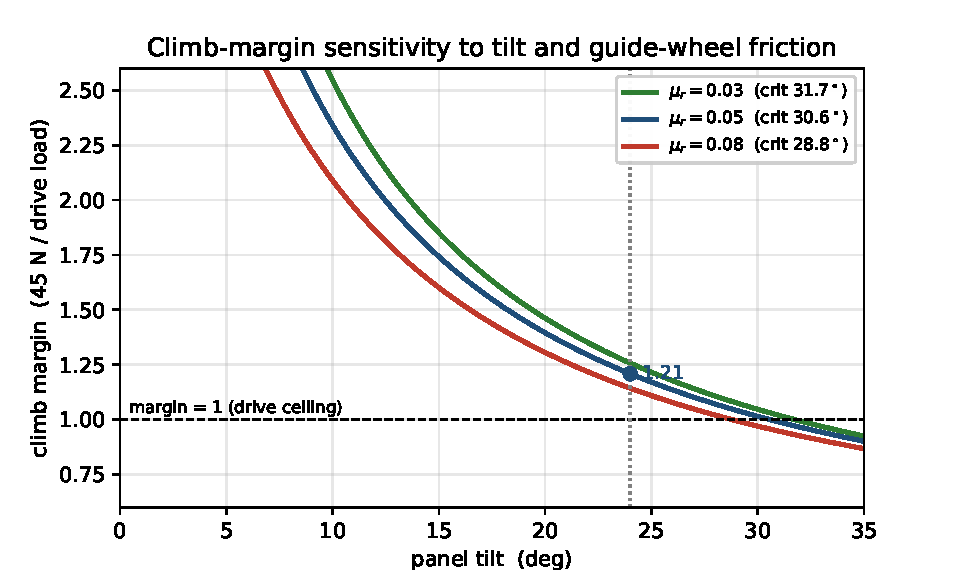
\includegraphics[width=0.82\linewidth]{fig_tilt_margin.pdf}
\caption{Climb margin vs.\ panel tilt for three guide-wheel friction values.
Dashed line: the \SI{45}{\newton} drive ceiling (margin $=1$). The design
\SI{24}{\degree} sits at \num{1.21}; the drive runs out near \SI{30}{\degree}.}
\label{fig:tilt}
\end{figure}

% ---------------------------------------------------------------
\shead{10.\ \ Three-scale deployment scaling}
The same per-tile harvesting physics and per-area cleaning duty scale linearly
across the three target deployments. Table~\ref{tab:scale} sizes each from the
model anchors: glass area at \SI{4.65}{\meter\squared\per\kilo\watt} (peak), a
light wash of \SI{0.3}{\liter\per\meter\squared} on a \SI{3.5}{\day} interval,
TEC tiles at \SI{0.106}{\liter\per\day} each, dock PV at
\SI{36}{\watt}\textsubscript{p} per tile, and one carriage servicing
\SI{518}{\meter\squared\per\day} at \SI{60}{\percent} field duty.

\begin{table}[h]\centering\small
\begin{tabular}{@{}l r r r r r r r r@{}}
\toprule
Variant & {kW\textsubscript{p}} & {Glass} & {L/event} & {L/day} & {TEC} & {Dock PV} & {Clean} & {Units} \\
        &        & {(m$^2$)} &        &        & {tiles} & {(kW\textsubscript{p})} & {(h)} & \\
\midrule
Commercial rooftop  & 200.0 & 929.5 & 278.8 & 79.7 & 752 & 27.0 & 8.61 & 1 \\
Residential rooftop & 9.9   & 46.0  & 13.8  & 3.9  & 38  & 1.36 & 0.43 & 1 \\
Street-lamp PV      & 0.3   & 1.4   & 0.42  & 0.12 & 2   & 0.07 & 0.01 & 1 \\
\bottomrule
\end{tabular}
\caption{Linear scaling of the validated residential model point (middle row,
\num{38} tiles / \SI{3.94}{\liter\per\day}) to the commercial and street-lamp
variants. The commercial AWG (\num{752} tiles, $\sim$\,\SI{27}{\kilo\watt}\textsubscript{p}) is
$\sim$\,\SI{13}{\percent} of the array it serves and would be a shared skid
feeding several carriages; the street-lamp case needs only a \num{2}-tile
micro-dock. Refine per real array layout (rail count, sub-arrays, local soiling
interval).}\label{tab:scale}
\end{table}

% ---------------------------------------------------------------
\shead{Validation --- computed vs.\ the model's stored values}
\begin{table}[h]\centering\small
\begin{tabular}{@{}l r r c@{}}
\toprule
Quantity & {Computed} & {Model JSON} & {Unit} \\
\midrule
Gravity force $F_g$            & 31.92 & 31.92 & \si{\newton} \\
Rolling force $F_r$            & 3.59  & 3.58  & \si{\newton} \\
Total drive force $F_\text{drive}$ & 37.24 & 37.23 & \si{\newton} \\
Required torque ($\times$1.5)  & 0.838 & 0.838 & \si{\newton\meter} \\
Pinion speed                   & 38.2  & 38.2  & \si{\rpm} \\
Drive mech.\ power             & 2.23  & 2.2   & \si{\watt} \\
Brush roller torque            & 0.043 & 0.043 & \si{\newton\meter} \\
Time per panel (down+up)       & 66.7  & 66.7  & \si{\second} \\
Water per event                & 0.60  & 0.60  & \si{\liter} \\
\bottomrule
\end{tabular}
\caption{First-principles results match the model's stored design values to
within rounding.}\label{tab:val}
\end{table}

\vspace{-0.2cm}
\noindent\colorbox{slideblue!8}{\parbox{\dimexpr\linewidth-2\fboxsep}{\small
\textbf{Headline numbers.}
Climb margin \textbf{1.21} on the \SI{24}{\degree} tilt;
drive-torque margin \textbf{1.86}; brush, gear and hold all amply sized.
Cleaning rate \textbf{\SI{108}{\meter\squared\per\hour}}
($\approx\SI{518}{\meter\squared\per\day}$ at \SI{60}{\percent} field duty).
Energy \textbf{\SI{0.89}{\watt\hour}} per panel $\Rightarrow$ \textbf{$\sim$108}
sweeps per battery charge.
\num{38}-tile dock harvests \textbf{\SI{4.03}{\liter\per\day}} $\ge$
\SI{3.94}{\liter\per\day} demand $\Rightarrow$ \textbf{water self-sufficient}
($f=1.02$).
Tip safety factor \textbf{4.9}.
All values reproduce \texttt{model\_calcs.py}; see \texttt{model\_calcs\_results.json}.}}

\end{document}
